% context: 9th-grade physics classwork, first problem set of the year
% topic: measurement, precision, significant figures, scientific notation, unit conversion
\documentclass[12pt, twoside]{article}
\input{../preamble}
\usepackage{float}

\title{Physics}
\author{Chris Huson}
\date{September 2026}

\fancyhead[LE]{\thepage}
\fancyhead[RO]{\thepage \\ Nickname: \hspace{2.25cm} \,\\ \,}
\fancyhead[LO]{La Scuola d'Italia / Huson / Physics \\* 10 September 2026}

\begin{document}

\subsubsection*{1.1 Classwork: Measurement, Precision, and Significant Figures}

\textbf{Reference (provided).} \quad 1 in. = 2.54 cm \quad 1 m $\approx$ 3.28 ft \quad 1 h = 3600 s \\
1 km = 1000 m \quad 1 m = 100 cm \quad 1 cm = 10 mm \quad 1 kg = 1000 g

\vspace{0.15cm}

\begin{enumerate}[itemsep=0.4cm]

\item Write down the number of significant digits in each measurement.
  \begin{multicols}{3}
    \begin{enumerate}[itemsep=0.35cm]
      \item 42
      \item 3.60
      \item 0.0058
      \item 0.01070
      \item 250.0
      \item 6.022
    \end{enumerate}
  \end{multicols} \vspace{0.35cm}

\item Round each value to three significant figures. Copy the calculator display followed by three dots, then round: $$\sqrt{2} = 1.4142135\ldots \approx 1.41$$
  \begin{multicols}{2}
    \begin{enumerate}[itemsep=1cm]
      \item The population of Milan: 1,371,498
      \item $\sqrt{5}$
    \end{enumerate}
  \end{multicols} \vspace{0.8cm}

\item The bar below is measured with a centimeter ruler marked in millimeters.

\begin{center}
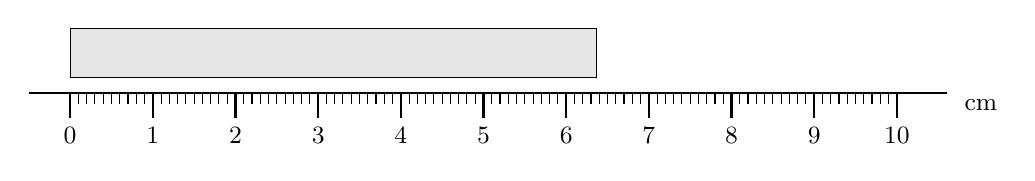
\begin{tikzpicture}[scale=1.05]
  \draw[fill=gray!20] (0,0.18) rectangle (6.37,0.78);
  \draw[thick] (-0.5,0) -- (10.6,0);
  \foreach \x in {0.1,0.2,...,9.95}{\draw (\x,0) -- (\x,-0.14);}
  \foreach \x in {0,1,2,3,4,5,6,7,8,9,10}{\draw[thick] (\x,0) -- (\x,-0.3) node[below] {\small \x};}
  \node[right] at (10.7,-0.15) {\small cm};
\end{tikzpicture}
\end{center}

  \begin{enumerate}[itemsep=0.9cm]
    \item Record the length of the bar. Include one estimated digit --- the last digit, the one you are not certain of.
    \item How many significant figures does your measurement have?
    \item Write the same length in millimeters, and again in meters.
  \end{enumerate} \vspace{0.9cm}

\item Write in scientific notation, rounded to three significant figures.
  \begin{multicols}{2}
    \begin{enumerate}[itemsep=1.3cm]
      \item The distance from New York to Rome: 6,890,000 meters.
      \item The diameter of a red blood cell: 0.0000078 meters.
    \end{enumerate}
  \end{multicols} \vspace{2cm}

\newpage

\item Write each value as an ordinary decimal number.
  \begin{multicols}{2}
    \begin{enumerate}[itemsep=1.2cm]
      \item $4.05 \times 10^{5}$ grams
      \item $2.9 \times 10^{-4}$ seconds
    \end{enumerate}
  \end{multicols} \vspace{1.6cm}

\item Convert between units, rounding to three significant figures. Write the conversion as a fraction and show the units cancelling.
  \begin{enumerate}[itemsep=2.2cm]
    \item The Colosseum stands 48.5 meters tall. What is its height in feet?
    \item A 12 inch ruler is how many centimeters long?
  \end{enumerate} \vspace{2cm}

\item A bus on Via del Corso travels at 30 kilometers per hour. What is this speed in meters per second? \vspace{3cm}

\item The mass of the Earth is $5.972 \times 10^{24}$ kg and the mass of Jupiter is $1.898 \times 10^{27}$ kg. How many times more massive is Jupiter than the Earth? Round to three significant figures. \vspace{2.5cm}

\item Challenge: Estimate the number of seconds you have been alive. Give your answer in scientific notation, and explain why it would be wrong to report this number to nine significant figures.

\end{enumerate}
\end{document}
